% =====================================
% Dies ist eine LaTeX-Vorlage für Masterarbeiten und vergleichbare Abschlussarbeiten bei Professor Bialonski.
% Die Vorlage ist aus einer bei Professor Bialonski durchgeführten Masterarbeit hervorgegangen.
% 
% Die Vorlage enthält einige Beispielinhalte, -tabellen und -abbildungen, an denen die Nutzung der verschiedenen Pakete und allgemeine LaTeX-Kommandos zur Ausarbeitung einer Abschlussarbeit zu sehen sind.
% Diese erheben weder einen Anspruch auf Vollständigkeit noch darauf immer den aktuell als Best Practice angesehenen Standards zu folgen.
% 
% Stellen, an denen Entscheidungen über Konfigurationen, verwendete Pakete etc. getroffen werden müssen sind mit einem TODO gekennzeichnet.
% =====================================

% =====================================
% Tipps:
%   für die Nutzung mit einem Versionsverwaltungssystem sollte mindestens mit jedem neuen Satz eine neue Zeile angefangen werden
%   bei der Nutzung des Babel-Pakets mit ngerman kann mit "= ein Bindestrich eingefügt werden, der es LaTeX erlaubt auch an anderen Stellen als dem Bindestrich einen Zeilenumbruch einzufügen, und mit "~ ein geschützter Bindestrich eingefügt werden, d.h. dieser darf nicht als Zeilenumbruch verwendet werden
%   bei der Verwendung z.B. von TeXstudio kann das LanguageTool eingebunden werden, siehe dazu auch https://paulomarconi.github.io/blog/LanguageTool%2BTeXstudio%2BVSCode/ und https://dev.languagetool.org/http-server
%   viele hilfreiche Tipps findet man hier: https://www.semipol.de/posts/2018/06/latex-best-practices-lessons-learned-from-writing-a-phd-thesis/
% =====================================


% Dokumentklasse
% TODO: Dies sind die wichtigsten Einstellungen, die vor Beginn des Schreibprozesses auf jeden Fall festgelegt werden sollten!
%       ich habe die KOMA-Script Abwandlung der report Klasse genutzt und kann dies auch im Nachhinein empfehlen
%       für allgemeine Informationen und Best Practices bezüglich der Auswahl der Schriftgröße und darauf basierend der Seitenränder empfiehlt es sich das Kapitel 2 der KOMA-Script Dokumentation (https://www.ctan.org/pkg/koma-script) zumindest zum Teil durchzulesen
%       ich finde den zweiseitigen Modus angebracht, dies kann allerdings auch zu weiteren Fragen bezüglich der Seitenränder etc. führen; wird der einseitige Modus genutzt, können eventuell die diversen \cleardoubleoddpage Befehle entfernt werden
%       die Bindungskorrektur wird von KOMA-Script dazu genutzt, den Verlust von Papier bei der Bindung in die Wahl der Seitenränder einzubeziehen, 10-12mm sind hier angebracht; für die reine Betrachtung als PDF wäre eigentlich eine Bindungskorrektur von 0 korrekt, dies würde allerdings zwei unterschiedliche Versionen mit ganz anderen Seitenrändern erfordern, von einer solchen Unterscheidung würde ich also abraten
%       DIV ist der Mechanismus der KOMA-Script Klassen für die Bestimmung der Breite der Seitenränder; ein guter Wert kann über "DIV=calc" berechnet werden und aus der log-Datei ausgelesen werden, anschließend kann man davon ausgehend leichte Änderungen vornehmen; für eine Schriftgröße von 12pt und einer Bindungskorrektur von 12mm ist 10 ein guter Wert; alternativ kann das geometry Paket verwendet werden, siehe dazu auch diverse weitere TODOs
\documentclass[
    12pt, % Schriftgröße
    twoside, % zweiseitiger Modus
    ngerman, % deutsches Dokument
    BCOR=12mm, % Bindungskorrektur
    DIV=11, % Division (Anzahl Spalten/Zeilen pro Seite, bestimmt implizit Margins)
    bibliography=toc, % Literatur zu Inhaltsverzeichnis hinzufügen
    openright
]{scrreprt}
%\usepackage{minted}

% Variablen bezüglich des Titels, Autors und Subjects
\newcommand{\titleDocument}{Optimization of German Text Simplification Models with Supervised Fine-tuning and Alignment Methods}
\newcommand{\authorDocument}{Ben Pietsch}
\newcommand{\subjectDocument}{Masterarbeit}
\newcommand{\locationDocument}{Jülich}
\newcommand{\dateDocument}{\today} % Alternativ z.B. 30.~September 2021

% grundsätzliche Informationen zum Dokument
\title{\titleDocument}
\author{\authorDocument}
\date{\dateDocument}

% Packete etc.
\usepackage{thesis}

\usepackage{lipsum}
\usepackage{textcomp}
\usepackage{wasysym} % TODO: nur für Beispieltext in summary.tex genutzt, wird nicht benötigt

%\usepackage[cache=false,outputdir=out]{minted}

% Besondere Trennungen (z.B. bei vereinzelter Nutzung englischer Begriffe ohne Nutzung des multilingualen Supports von babel)
\hyphenation{Kon-fi-denz Kon-fi-denz-wert Mus-kel-ak-ti-vi-tät O-pen-Shift Platt-form-en}

\makeglossaries
\newglossaryentry{axa}{
    name=AXA Konzern AG,
    description={Die AXA Konzern AG~\autocite{axa} ist die deutsche Tochtergesellschaft des französischen Versicherungsunternehmens
    AXA und gehört mit über sieben Millionen Kunden zu den größten Versicherungen Deutschlands}
}

\newglossaryentry{illit}{
    name=functional illiterates,
    description={TODO}
}

\newacronym{nls}{NLS}{Netzwerk Leichte Sprache}
\newacronym[first={Easy Language (in German: \enquote{Leichte Sprache})}]{el}{EL}{Easy Language}
\newacronym[first={Plain Language (in German: \enquote{Einfache Sprache})}]{pl}{PL}{Plain Language}
\newacronym{bgg}{BGG}{Act on Equal Opportunities of Persons with Disabilities (in German: Behindertengleichstellungsgesetz)}



% Abkürzungen
% Beispiele für Verwendung von Akronymen; standardmäßig ist first als "long (short)" definiert
\newacronym{cnn}{CNN}{Convolutional Neural Network}
\newacronym[first={Kreuzvalidierung (engl. Cross Validation, CV)}]{cv}{CV}{Cross Validation}

% keine Worttrennungen in Abkürzungen
% könnte mit Sicherheit auch automatisiert werden aus der obigen Liste, habe ich nicht ausprobiert
\hyphenation{CNN CV}

\begin{document}
    % ============ Anfang =============
    % Titelseite
    \pagenumbering{roman}
    \begin{titlepage}
	% TODO: wird das geometry Paket genutzt statt der Mechanismen aus KOMA-Skript, kann die folgende Zeile z.B. durch "\newgeometry{...}" ersetzt werden
	\typearea{100} % DVI auf 100 setzen für Titel (kleine Margins)
	\setlength{\parindent}{0pt} % keine Einrückung bei neuen Absätzen auf dieser Seite
	
	\begin{flushright}
		
\includegraphics[height=5cm]{images/FH-Aachen-r_svg-raw}
	\end{flushright}
	
	\vspace*{-2.5cm}

	\begin{center}
		\textbf{\Huge Fachhochschule~Aachen}

		\vspace*{0.5cm}
		
		\textbf{\Huge Campus~Jülich}

		\vspace*{0.75cm}

		{\normalsize\doublespacing Fachbereich~9:~Medizintechnik~und~Technomathematik\\	Studiengang:~Angewandte~Mathematik~und~Informatik}

		\vspace*{2.0cm} % TODO: bei mehr verwendeten Zeilen für den Titel verringern
		
		\begin{minipage}[t]{17cm} % TODO: abhängig von dem konkreten Titel muss diese Breite eventuell angepasst werden für einen passenden Zeilenumbruch
			\begin{center}
				\textbf{\Huge \titleDocument}
			\end{center}
		\end{minipage}
	
		\vspace*{2.0cm} % TODO: bei mehr verwendeten Zeilen für den Titel verringern (symmetrisch zu oben)
		
		\textbf{\Large \subjectDocument}

		\vspace*{0.1cm}
		
		{\normalsize von}
		
		\vspace*{0.5cm}
		
		\textbf{\Large \authorDocument}
	
		\vspace*{3.5cm}
		
		\begin{minipage}[t]{13cm}
			\begin{center}
				\begin{tabular}{ll}
					Erstprüfer: & Prof. Dr. rer. nat. Bodo Kraft \\
					Zweitprüfer: & M.Sc. Lars Klöser \\
					Matrikelnummer: & 3237534 \\
				\end{tabular}
			\end{center}
		\end{minipage}
		
		\vspace*{2.5cm}
	
		{\large \locationDocument, \dateDocument}
	\end{center}
\end{titlepage}

% TAN BA: 0558.3483.9284
    \cleardoublepage

    % Eidesstattliche Erklärung und Abstrakt
    \begingroup

    % keine Seitenzahl und kein running header
        \thispagestyle{empty}
        \renewcommand*{\chapterpagestyle}{empty}


        \cleardoubleoddpage % Eidesstattliche Erklärung rechts, damit Unterschrift nicht durchdrückt
        \chapter*{Eidesstattliche Erklärung} % kein Eintrag im Inhaltsverzeichnis

Ich versichere hiermit, dass ich die vorliegende Masterarbeit mit dem Thema
\begin{quote}
    \textit{\titleDocument}
\end{quote}
selbstständig verfasst und keine anderen als die angegebenen Quellen und Hilfsmittel benutzt habe, wobei ich alle wörtlichen und sinngemäßen Zitate als solche gekennzeichnet habe.
Die Arbeit wurde bisher keiner anderen Prüfungsbehörde vorgelegt und auch nicht veröffentlicht.

\vspace*{2cm}

\begingroup
\setlength{\parindent}{0pt} % keine Einrückung bei neuen Absätzen in diesem Bereich

\locationDocument, den \dateDocument
\bigskip
\bigskip

% gewünschte Breite der Unterschriftslinie
\newlength{\widthbox}
\settowidth{\widthbox}{\locationDocument, den \dateDocument}

\makebox[\widthbox]{\hrulefill}\\
\authorDocument
\endgroup

        \cleardoubleoddpage % Abstrakt rechts
%        \pagestyle{emtpy}
        \chapter*{Abstract} % kein Eintrag im Inhaltsverzeichnis

%In diesem Kapitel wird die Arbeit kurz und prägnant in maximal einer Seite zusammengefasst.
%Ein klassisches Abstrakt beinhaltet die nachfolgenden Punkte:
%\begin{enumerate}
%	\setlength{\itemsep}{0pt}
%	\item Die Relevanz des betrachteten Themas erläutern. (allgemein/umfassend)
%	\item Die wichtigsten Herausforderungen aufführen und dadurch die Arbeit motivieren.
%	\item Diese Untersuchungen wurden durchgeführt. (knapp)
%	\item Die erhaltenen Resultate wiedergeben.
%	\item Die daraus folgenden Konsequenzen und eventuelle weitere Schritte diskutieren. (allgemein/umfassend)
%\end{enumerate}
%Wie an dem Inhalt der Klammern in der Auflistung zu erkennen ist, besitzt das Abstrakt eine Sanduhr-Struktur, \ie{} der Mittelteil wird sehr knapp bzw. spezifisch abgehandelt, während der Anfang und das Ende allgemeiner bzw. umfassender erläutert werden.
%
%Akronyme wie \zB{} \gls{cnn}, die bereits im Abstrakt verwendet werden, werden durch den Befehl \enquote{glsresetall} im Root-Dokument für den Hauptteil zurückgesetzt.

        \glsresetall % alle bereits genutzten Akronyme wieder zurücksetzen
    \endgroup

    % Inhaltsverzeichnis
    \cleardoubleoddpage % Inhaltsverzeichnis rechts
    \begingroup
        \hypersetup{hidelinks}
        \pagestyle{empty}
        \tableofcontents
        \addtocontents{toc}{\protect\thispagestyle{empty}}
        \listoffigures
        \thispagestyle{empty}
    \endgroup
    % =========== Hauptteil ===========
    \cleardoubleoddpage % Beginn Einleitung rechts
    \pagenumbering{arabic}
    \chapter{Introduction}\label{ch:introduction}

In the digital age written text has become ubiquitous. % (TODO: cite?~\autocite{salar-mohtaj-babak-naderi-2022-overview})
% TODO: Examples for important written text: Websites, Online Messages like E-Mails, Newspapers, Government Authorities (distribute Information)

Today the ability to comprehend text is a necessary prerequisite to actively participate in society. % nowadays
This poses a challenge to people with communication impairments~\autocite{easyLanguageBook}.
In Germany, about 12\% of the population has difficulties to understand and write standard german because of reduced literacy~\autocite{schomacker2023data}.
Complicated texts can act as a barrier which prevents these people from taking part in everyday life~\autocite{easyLanguageBook}
% could lead to exclusion,

Several attempts have been made to create a type of written language that is more comprehensible and accessible.
The primary goal of such languages is to improve communication for a broad range of people with limited reading and writing skills.
This group includes people with communication impairments, people with dementia, language learners, \gls{illit} and older people with visual impairments~\autocite{easyLanguageBook}.

In German, two simplified languages have gained popularity in recent years: \enquote{Easy Language} and \enquote{Plain Language}.

%The simplified language has to be simple enough to be understood by everyone.
%At the same time it should not be impractical for people that are proficient in standard language.


\section{Easy Language}\label{sec:el}

\gls{el} is a type of simplified language that is regulated by a set of rules.
There are multiple guidelines published by different organizations that define those rules.
The most commonly used guideline is distributed by the \enquote{\gls{nls}}~\autocite{netzwerkLS, easyLanguageBook}.

The \gls{nls} was founded in 2006 and became an official association in 2013~\autocite{netzwerkHistory}.
The association aims to popularize and standardize \gls{el} in Germany.
All members are volunteers~\autocite{netzwerkGoals}.
Among others, the \gls{nls} includes the following people in their target group:
\begin{itemize}[noitemsep]
    \item people with learning difficulties
    \item people with the illness dementia
    \item people that are not proficient in German
    \item people with reduced reading abilities
\end{itemize}
The \gls{nls} intends that texts written in \gls{el} are verified by certified examiners.
Examiners are trained at the \gls{nls} and are usually people in the target group~\autocite{netzwerkPruef}.

\subsection{Rules and Recommendations}\label{subsec:el-rules}
The rules for \gls{el} fall into the categories \enquote{Words}, \enquote{Numbers and Symbols}, \enquote{Sentences}, \enquote{Content} and \enquote{Presentation and Images}.

Words are supposed to be simple.
Technical and foreign words should be avoided.
If difficult words are unavoidable, they have to be explained.
Once a word was introduced to describe a subject, that word should be used again when the subject is referred to.

\begin{figure}[htb]
    \begin{center}
        \colorbox{badred!20}{
            \begin{minipage}{0.6\textwidth}
                \fontfamily{pag}
                A car drove past me.\\
                It was very fast.\\
                The vehicle was red.
            \end{minipage}
        }
        \colorbox{goodgreen!20}{
            \begin{minipage}{0.6\textwidth}
                \fontfamily{pag}
                A car drove past me.\\
                It was very fast.\\
                The car was red.
            \end{minipage}
        }
    \end{center}
    \caption[Using the same word to refer to the same subject.]{Using the same word to refer to the same subject (bottom). Using synonyms can be confusing (top).}
    \label{fig:subject_ref}
\end{figure}
Shorter words are preferred over longer words.
If long words are necessary, they should be split with a hyphen character (e.g.\ \enquote{Bundes-Gleichstellungs-Gesetz} instead of \enquote{Bundesgleichstellungsgesetz}).
Additional rules for words are
\begin{itemize}[noitemsep]
    \item the avoidance of acronyms
    \item the use of active voice over passive voice
    \item avoidance of genitive and conjunctive
    \item reduced use of negation
\end{itemize}
Numbers and symbols are another aspect that is addressed by the \gls{nls}-guideline.
Numbers should be written in arabic numerals.
For many people digits are easier to read than the spelled out word (e.g.\ \enquote{5 horses} instead of \enquote{five horses}).#
Thus, smaller numbers are to be witten in digits.
Very large numbers are replaced by rough estimations (e.g.\ \enquote{Many People} instead of \enquote{14.795 People}).
The same goes for percentages.
If unusual symbols (e.g.\ §) are used they need to be explained.

The structure of sentences has a big impact on readability. % TODO: quelle?
In \gls{el} sentences are supposed to be short.
Every sentence should only include one statement.
After each sentence a new line is started.
Sentences with simple structures like \enquote{subject, verb, object} are preferred.
More complex sentences should be broken up in smaller pieces.
These smaller pieces do not necessarily need to form a complete sentence.
\begin{figure}[htb]
    \begin{center}
        \colorbox{badred!20}{
            \begin{minipage}{0.6\textwidth}
                \fontfamily{pag}
                Do you want to go swimming or watch a movie?
            \end{minipage}
        }
        \colorbox{goodgreen!20}{
            \begin{minipage}{0.6\textwidth}
                \fontfamily{pag}
                Do you want to go swimming? \\
                Or watch a movie?
            \end{minipage}
        }
    \end{center}
    \caption[Splitting longer sentences in \glsentrylong{el}.]{Splitting longer sentences in \glsentrylong{el}. To comply with the rules of \gls{el} the (top) sentence is split in two. The second part of the (bottom) example does not form a complete sentence on its own.}
    \label{fig:split_sentence}
\end{figure}
%\begin{mybox}{Bad example}
%    Do you want to go swimming? \\
%    Or watch a movie?
%\end{mybox}
Sentences with subordinate clauses can be broken up similarly.

Topics should not be distributed across the text.
Related content should be kept together.
References to other texts are to be avoided.
In the translation process from standard German to \gls{el} content can be omitted if necessary.
Likewise, additional content can be added to make the text more understandable.

The presentation of text is another aspect that impacts clarity and readability.
The \gls{el}-guideline recommends using a big font size and big line spacing.
Furthermore, text is to be left-aligned.
Backgrounds are supposed to be in light color while the written text is colored darkly.
Text should be structured in many paragraphs with frequent headlines.
Using bullet points instead of comma separated enumerations improves clarity.
Images can be added to accompany the text~\autocite{netzwerkLS}.

\subsection{Prevalence and Adoption of Easy Language}\label{subsec:el-adop}

\glsentrylong{el} contains features that go against standard german.
The unique layout with very short lines makes it easy to recognize texts in \gls{el}.
This helps the target group to find texts written in \gls{el} easily.
But the strong divergence from standard German has been repeatedly criticised.
In 2015, the Federal State Parliament of Schleswig-Holstein passed a law to make elections more accessible.
Information regarding elections was sent out to all voters in \gls{el}.
This sparked outrage in the population and was denounced by multiple politicians.
As a result the passed law was reverted~\autocite{easyLanguageBook}.

While \gls{el} has yet to find acceptance in the general population, it has already been incorporated into german law.
In 2002 the \gls{bgg} was adopted.
The \gls{bgg} guarantees equal living conditions to people regardless of disabilities.
In 2018 the \gls{bgg} was extended to include clearer instructions for accessibility~\autocite{bggInfo}.
Since then, public authorities have to provide information in \gls{el} as specified in section 2, paragraph 11~\autocite{bgg2018}.
Today \gls{el} can be found on many websites of government departments and municipal institutions (e.g.\ the City Cologne: \url{https://www.stadt-koeln.de/artikel/07808/index.html}).

\begin{figure}
    \centering
    \colorbox{goodgreen!20}{
        \begin{minipage}{0.6\textwidth}
            Fische sind Tiere. \\
            Sie leben im Wasser. \\
            In Flüssen, im Meer und in Seen. \\
            \\
            Fische atmen durch Kiemen. \\
            Das ist ein Körper-teil. \\
            Dadurch können sie unter Wasser atmen.
        \end{minipage}
    }
    \caption[Text written in \glsentrylong{el}.]{Text written in \gls{el} taken from the online dictionary \enquote{Hurraki} (\url{https://hurraki.de/wiki/Fische}).}
    \label{fig:easy_text}
\end{figure}


\section{Plain Language}\label{sec:pl}
\gls{pl} is a simplified language that is much closer to standard language.
Originally, it was not intended for people with disabilities.
\gls{pl} is often used to explain domain-specific texts in expert language to less informed people.
Moreover, it addresses language learners, e.g.\ migrants and people that learn German as a second language~\autocite{easyLanguageBook}.

In the English language guidelines for \gls{pl} have existed for a long time.
Some early works on more accessible language were published in the beginning of the 20th century.
From the 1960s on the US government pushed to propagate the use of \gls{pl}.
The goal was to improve communication between citizens and experts from administrative institutions.
Several instruction manuals for \gls{pl} were distributed.
Since 2010 federal agencies in the US are required to offer information in a form that is well understood by the citizens.

In Germany efforts for \gls{pl} have only been made very recently.
In the 1980s \enquote{Bürgernahe Sprache} (in English: \enquote{language that is close to the citizens}) was created to make administrative texts more comprehensible.
\enquote{Bürgernahe Sprache} does not take people with communication impairments and less educated people into account.
Thus, it does not satisfy all expected conditions of a simplified language.
In the 2000s multiple approaches for \gls{pl} with a broader target groups were attempted.
But none of them have been widely accepted as a standard yet.
Typical features of \gls{pl} are
\begin{itemize}[noitemsep]
    \item use of common words
    \item use of short words
    \item avoidance of ambiguous words
    \item precise formulations
    \item short sentences
    \item active voice
    \item clear sentence structure (e.g.\ a maximum of two subordinate clauses)
    \item avoidance of acronyms
\end{itemize}
These directives are similar to some rules in the \gls{el}-guideline.
But \gls{pl} does not break any rules of standard German.
That might be a reason why \gls{pl} is generally viewed in a more positive light than \gls{el} by many people. % viewed favorably
Moreover, \gls{pl} can be more flexible and less restrictive as there are no fixed rules.
Writers of \gls{pl} are supposed to factor in the audience of the text and make changes accordingly~\autocite{easyLanguageBook}.

\begin{figure}
    \centering
    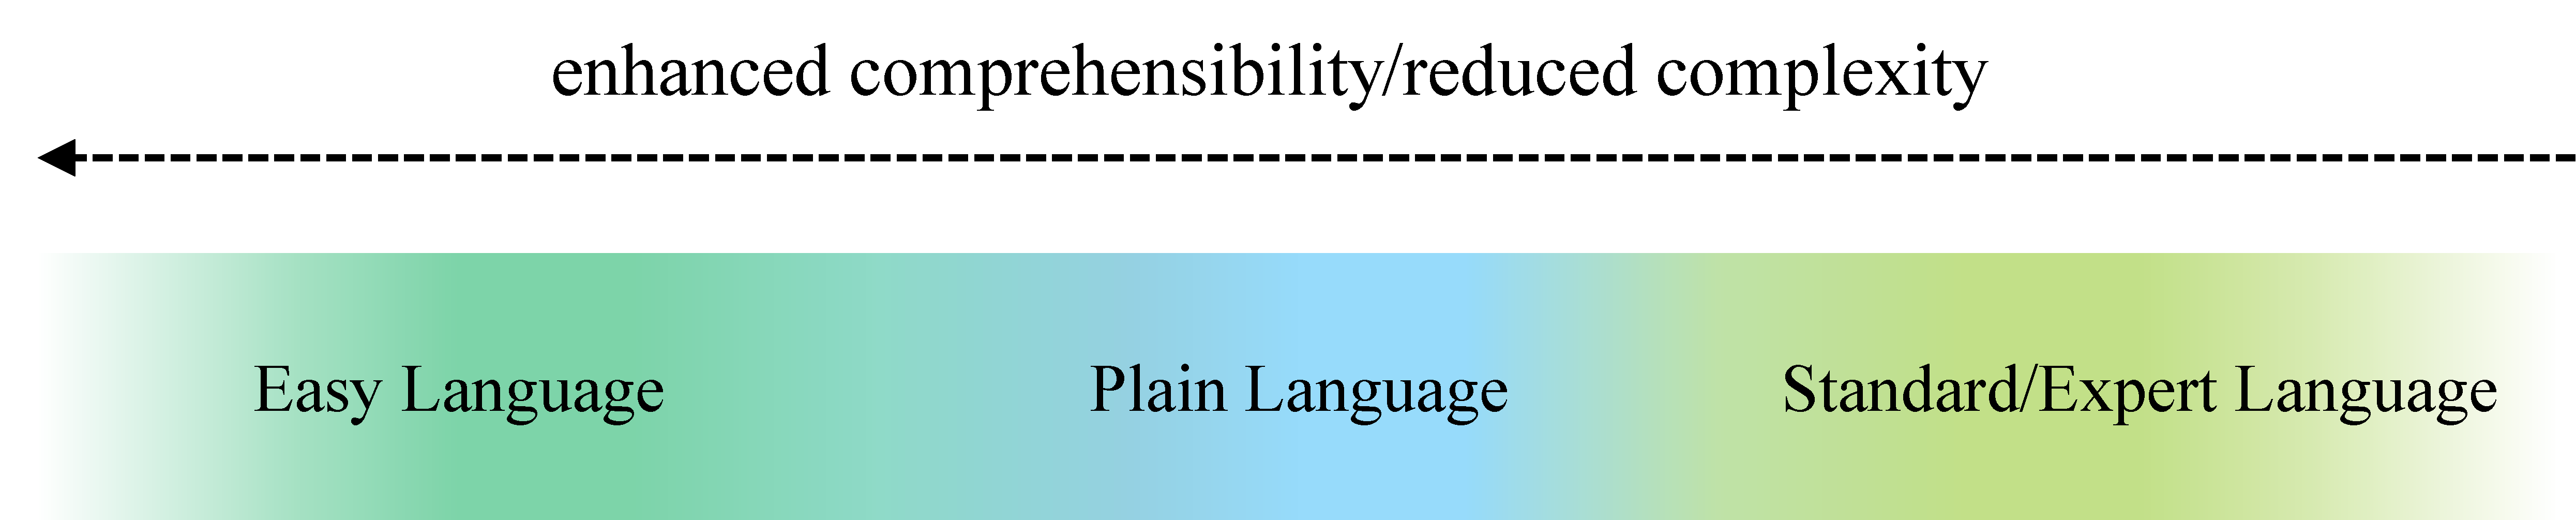
\includegraphics[width=\linewidth]{images/easy_languages}
    \caption[Different levels of text complexity and comprehensibility.]{Different levels of text complexity and comprehensibility. The different types of languages overlap in certain aspects~\autocite{easyLanguageBook, selbsterstellt}}
    \label{fig:languages}
\end{figure}


 % TODO: CEFR, UN, (BITV 2.0)
%\section{Terminologie}\label{sec:term}

%ambiguity of terminology

%    more difficult to understand than easy language
%
%
%From~\autocite{un2008}:
%Article 9 -Accessibility: "sinage in easy to read and understand forms", "ensure access to information"
%
%Article 2: plain-language listed under communication
%
%Article 29 - Participation in political and public life

%easy, plain, simple with very similar meanings

%    different guidelines:
%        inclusion europe
%        Netzwerk Leichte Sprache -> most commonly used
%        Barrierefreie-Informationstechnik-Verordnung (BITV 2.0)
%
%    rulebooks published by Duden


%

%From~\autocite{schomacker2023data}:
%"Easy language is roughly equivalent with level A2 of the Common European Framework of Reference for Languages (CEFR)"

\section{Automatic Language Simplification}\label{sec:langSimp}

Writing texts in \gls{pl} or \gls{el} and translating complex texts into simpler forms requires much effort~\autocite{easyLanguageBook}.
Hence, there is a demand for tools that can assist in this process.
In the context of \gls{nlp} the task of computer aided reduction of text complexity is known as \gls{ats}~\autocite{Ansch_tz_2023}.
The goal of \gls{ats} is to create a system that takes a text in standard or expert language as an input and outputs a simplified version of that text.
\gls{ats} is similar to other \gls{nlp}-tasks like summarization~\autocite{rios-etal-2021-new} and language translation~\autocite{aumiller2022klexikon}.
It is a \gls{seq2seq}-task~\autocite{Ansch_tz_2023} meaning the desired system has to processes and output texts of varying lengths.
\gls{ats} is a relatively new \gls{nlp}-task~\autocite{schomacker2023data}.
Especially simplification of German text has not seen a lot of research~\autocite{Ansch_tz_2023}.

Some \gls{ats}-methods focus only on sentence-level simplifications while other approaches aim to simplify whole documents.
Simplifications on sentence-level have the advantage that the \gls{ats}-System has to perform less complex transformations on the text.
But certain features of \gls{el} like the organization of content order and structure (see section~\ref{subsec:el-rules}) cannot be taken into account. %TODO: Braucht das eine quelle oder ist das offensichtlich?
Document-level simplifications do not have this problem.
However, they require the \gls{ats}-system to be able to process longer sequences and to carry out very complex modifications.

An early rule-based approach for language simplification into \gls{el} was presented by~\autocite{suter2016}.
This approach employed dictionaries to substitute difficult symbols.
Sentences and long words were split through a defined rule-set and additional explanations were added by inserting entries from the online dictionary \enquote{Hurraki}.
~\autocite{Garain2019} created another rule-based method using parse-trees to simplify english sentences.

Solutions based on \enquote{Deep Learning} are generally superior to rule-based methods for language translation tasks.
However, they require vast amounts of data~\autocite{otter2019survey}.
The data is usually a collection of texts (known as a \enquote{corpus}) which are related to the task at hand.
In the setting of language translation \enquote{parallel data} is very useful.
A parallel corpus contains pairs of source and target texts that function as an example for the task.
For \gls{ats} a parallel example would consist of a source text in standard language and a corresponding simplification.
Creating a parallel corpus is difficult as source and target text need to be properly aligned.
It is much easier to assemble a monolingual corpus that usually only contains texts in the target language~\autocite{chan2023routledge}.
While these monolingual corpora are less optimal than parallel data they can still be used in various ways to improve machine translation systems~\autocite{lample2018unsupervised, burlot2019using, chan2023routledge}.

Unfortunately, data for german language simplification is scarce~\autocite{Ansch_tz_2023}.
Most recent research has focused on creating corpora for \gls{el} and \gls{pl} to make Deep Learning approaches more feasible.

\textcite{klaper-etal-2013-building} build the first parallel corpus for german text simplification that consists of 256 texts~\autocite{ebeling2022}.
This corpus was later extended by~\textcite{battisti-etal-2020-corpus}.
The texts were extracted from PDF files and websites.
The extended corpus includes 6,217 documents of which the majority are monolingual (i.e.\ simplifications only) and is referred to as the \enquote{Web-Corpus} by~\textcite{ebeling2022}.
\textcite{sauberli-etal-2020-benchmarking} gather parallel data from news items provided by the \enquote{Austria Presse Agentur} (APA) that were manually simplified under the guidelines of \gls{capito}.
All in all the \enquote{APA-Corpus} contains 2,426 distinct documents~\autocite{ebeling2022}.
The data is then used to train \gls{ats}-models for sentence-level simplifications using the transformer architecture (see section~\ref{sec:trans}). %TODO: first neural simplification approach based on transformers, "lack of fluency and content preservation" (~\autocite{Ansch_tz_2023})
This is possibly the first transformer-based approach to german \gls{ats}~\autocite{Ansch_tz_2023}.
The company \gls{capito} also built a parallel corpus of about 1000 documents that is not publicly available~\autocite{ebeling2022}.

All the above-mentioned datasets contain a mix of different simplification levels.
Moreover, due to copyright issues, most of the data is not easily accessible~\autocite{stodden-etal-2023-deplain}.

\textcite{rios-etal-2021-new} create and publish a parallel document-level corpus from articles of the Swiss news magazine \enquote{20 Minuten} containing 17,905 article pairs.
The simplifications are written in \gls{pl} and are strongly summarized.
They train transformer-based language models on the published dataset while also including the \enquote{Capito Corpus} and the \enquote{APA Corpus}.

Another transformer-based approach for \gls{ats} is presented by~\textcite{spring-etal-2021-exploring}.
Their models are also trained on the corpora \enquote{Capito} and \enquote{APA} and can output different levels of simplified language based on the \gls{cefr}.


%\enquote{Deep Learning} is a subset of \enquote{Machine Learning}~\autocite{jagdaleDeepLearning2022}.


\section{Notes}\label{sec:notes}



From~\autocite{naderi2019subjective}
TextComplexityDE: 250 parallel sentences

From~\autocite{aumiller2022klexikon}:
German children’s encyclopedia \enquote{Klexikon} aligned with article from Wikipedia in standard language
exploring the task of simultaneous simplification and summarization

From~\autocite{deilen2023using}
Using sota model ChatGPT-3.5 to prompt for translations into \gls{el}
Outputs text that are easier to understand but leaving out information and not following the rules of \gls{el}

From~\autocite{toborek2023new}:
scrapers for different websites
automatic sentence alignment of parallel documents
corpus of 708 aligned documents


From~\autocite{Ansch_tz_2023}:
data for german language simplification is scarce
pretraining causal language models improves ATS performance
using monolingual Easy Language Data to fine-tune a GPT-like models
-> decoder output in style of \gls{el}
training ATS task on pretrained mBart model (replacing decoder with above-mentioned GPT-like Decoders, trainig cross-attention only)
publish web scraper for different website with easy language

From ~\autocite{stodden-etal-2023-deplain}
DEPlain corpus

From~\autocite{klöser2024german}:
previous work
using ChatGPT to generate standard language from monolingual \gls{el} and \gls{pl} to form synthetic parallel data
show that rule-based evaluations for \gls{el} are limited
evaluation of this seq2seq task is very difficult

back-translation (~\autocite{sennrich-etal-2016-improving})




% TODO: Evaluation
%From~\autocite{madina2023easytoread} TODO: Survey
%From~\autocite{salar-mohtaj-babak-naderi-2022-overview}: TextComplexity 2022

BLEU: ~\autocite{papineni-etal-2002-bleu}
SARI: ~\autocite{xu-etal-2016-optimizing}

    \chapter{Large Language Models}\label{ch:techOverview}

Creating machines with human-like language understanding has been a subject of research since the 1950s.
\gls{natural-language}s are highly complex and pose a difficult challenge to computers.
% ambiguous: ~\autocite{quadarLM2020}
\gls{lm} is an approach to make machines read, write and communicate like humans~\autocite{zhao2023survey}.

The main idea of \gls{lm} is to estimate probability distributions over units of texts, e.g.\ words~\autocite{de2015survey}.
Assuming that the occurrence of a word depends on previous words, i.e.\ the context, the probability of that word being next in a sentence can be modeled with a conditional probability~\autocite{jozefowicz2016exploring}.
\[
    P(w_n | w_1, \dots , w_{n-1})
\]
% TODO: quelle finden vielleicht
The ability to estimate the probability distributions over words makes it possible to predict the next word for a given sequence.
In this way, language models can be applied in many \gls{nlp} tasks like speech recognition, machine translation and text summarization~\autocite{jozefowicz2016exploring}.
By simply predicting the next word, language models can hold human-like conversations, which makes it appear as if they understand natural language.
% How would translation look like?
% TODO: Other approaches like BERT Masked language Modeling
%Other approaches to \gls{lm} mask parts of sentences and use all surrounding language units to predict the missing

There are different techniques to model these probabilities of word sequences.
In the 1990s, \glspl{slm} found widespread use.
The models often assume that the distribution of a word only depends on a fixed length of previous words.
\enquote{$n$-grams models} are \glspl{slm} that use the previous $n$ words to calculate the probability distribution of the next word.
Based on a training corpus, tables of conditional probabilities are created.
The probabilities are approximated by counting occurrences of $n$-grams.
If the previous word is \enquote{thank}, the probability that the next word is \enquote{you} could be estimated as follows~\autocite{quadarLM2020}
\[
    P(\text{you} | \text{thank}) = \frac{P(\text{thank you})}{P(\text{thank})} \approx \frac{count(\text{thank you})}{count(\text{thank})}
\]
In recent years, research has been focused on the more flexible \glspl{nlm}~\autocite{quadarLM2020}.
This approach uses \glspl{dnn} to estimate the needed probability distributions.
\glspl{nlm} are much better at taking long-range depencies in text into account than \glspl{slm}~\autocite{Hadi_2023}.
\glspl{dnn} excel at extracting complex features from text and finding meaningful representations for words.
These representations (often called embeddings) lie in a vector space of real vectors where similar words are close to each other in a mathematical sense~\autocite{quadarLM2020}.
In \glspl{nlm} the prediction function is usually built on top of these embeddings.
The intermediate step of learning effective features and representing them in embeddings has the benefit that those embeddings can be reused for other tasks.
The early 2010s saw the rise of \glspl{dnn} that were specifically designed to create powerful word embeddings~\autocite{zhao2023survey}.
These embeddings were static, meaning the network would assign each word exactly one embedding, disregarding polysemy of words~\autocite{Liu_2020}.
Embeddings of popular solutions like \enquote{word2vec} proved to be very useful in various \gls{nlp}-Tasks.

Following research focused on incorporating context into word embeddings, i.e.\ assigning a different vector representation to a word depending on the surrounding words.
ELMo, BERT and GPT are well-known models that managed to do so.
These context-aware language models are trained on large unlabeled corpora of text data.
During training, the models learn to solve pre-training tasks that are specifically designed for the language model to gain essential language understanding.
They are often put into their own class of language models, the so-called \glspl{plm}.
\glspl{plm} set new standards in solutions of many \gls{nlp}-tasks.
They learn general-purpose features that can be effectively used by fine-tuning the models on downstream tasks, e.g.\ machine translation, text summarization or \gls{ats}.
The process of using a \gls{plm} as a base model to fine-tune it for a specific task has become a commonly used pattern in \gls{lm}~\autocite{zhao2023survey}.

The availability of huge datasets and powerful computing devices led to another evolution in \gls{lm}.
\glspl{llm} are \glspl{plm} that are scaled in model size.
They are usually based on the popular transformer architecture~\autocite{Hadi_2023} and consist of billions of parameters.
Research found that using larger models with more extensive pre-training on larger datasets greatly improves performance~\autocite{Raiaan2024ARO}.
\glspl{llm} even show unexpected abilities (called emergent abilities) that could not be observed in smaller models, e.g.\ reasoning and solving complex tasks without fine-tuning~\autocite{zhao2023survey}.
They are capable of \enquote{in-context learning} meaning they can perform tasks given only instructions and a few examples without the need of updating model parameters~\autocite{bhatia2023tart}.
ChatGPT is an example of a popular \gls{LLM} with amazing conversation and task solving abilities~\autocite{zhao2023survey}.

While \glspl{llm} produce impressive results with \enquote{in-context learning} they are usually still outperformed by fine-tuned language models in specific tasks~\autocite{bhatia2023tart}.
In the context of German \gls{ats} this is supported by the results of~\textcite{deilen2023using} who find that ChatGPT can only create very rudimentary simplifications.

The course of action for this thesis is to use pre-trained base models to fine-tune them on the task of \gls{ats}.
Due to hardware limitations, only \glspl{plm} with up to 13 billion parameters come into question.
In the following sections the underlying workings of \glspl{nlm}, \glspl{plm} and \glspl{llm} will be explained.

% TODO
\begin{figure}
    \centering
    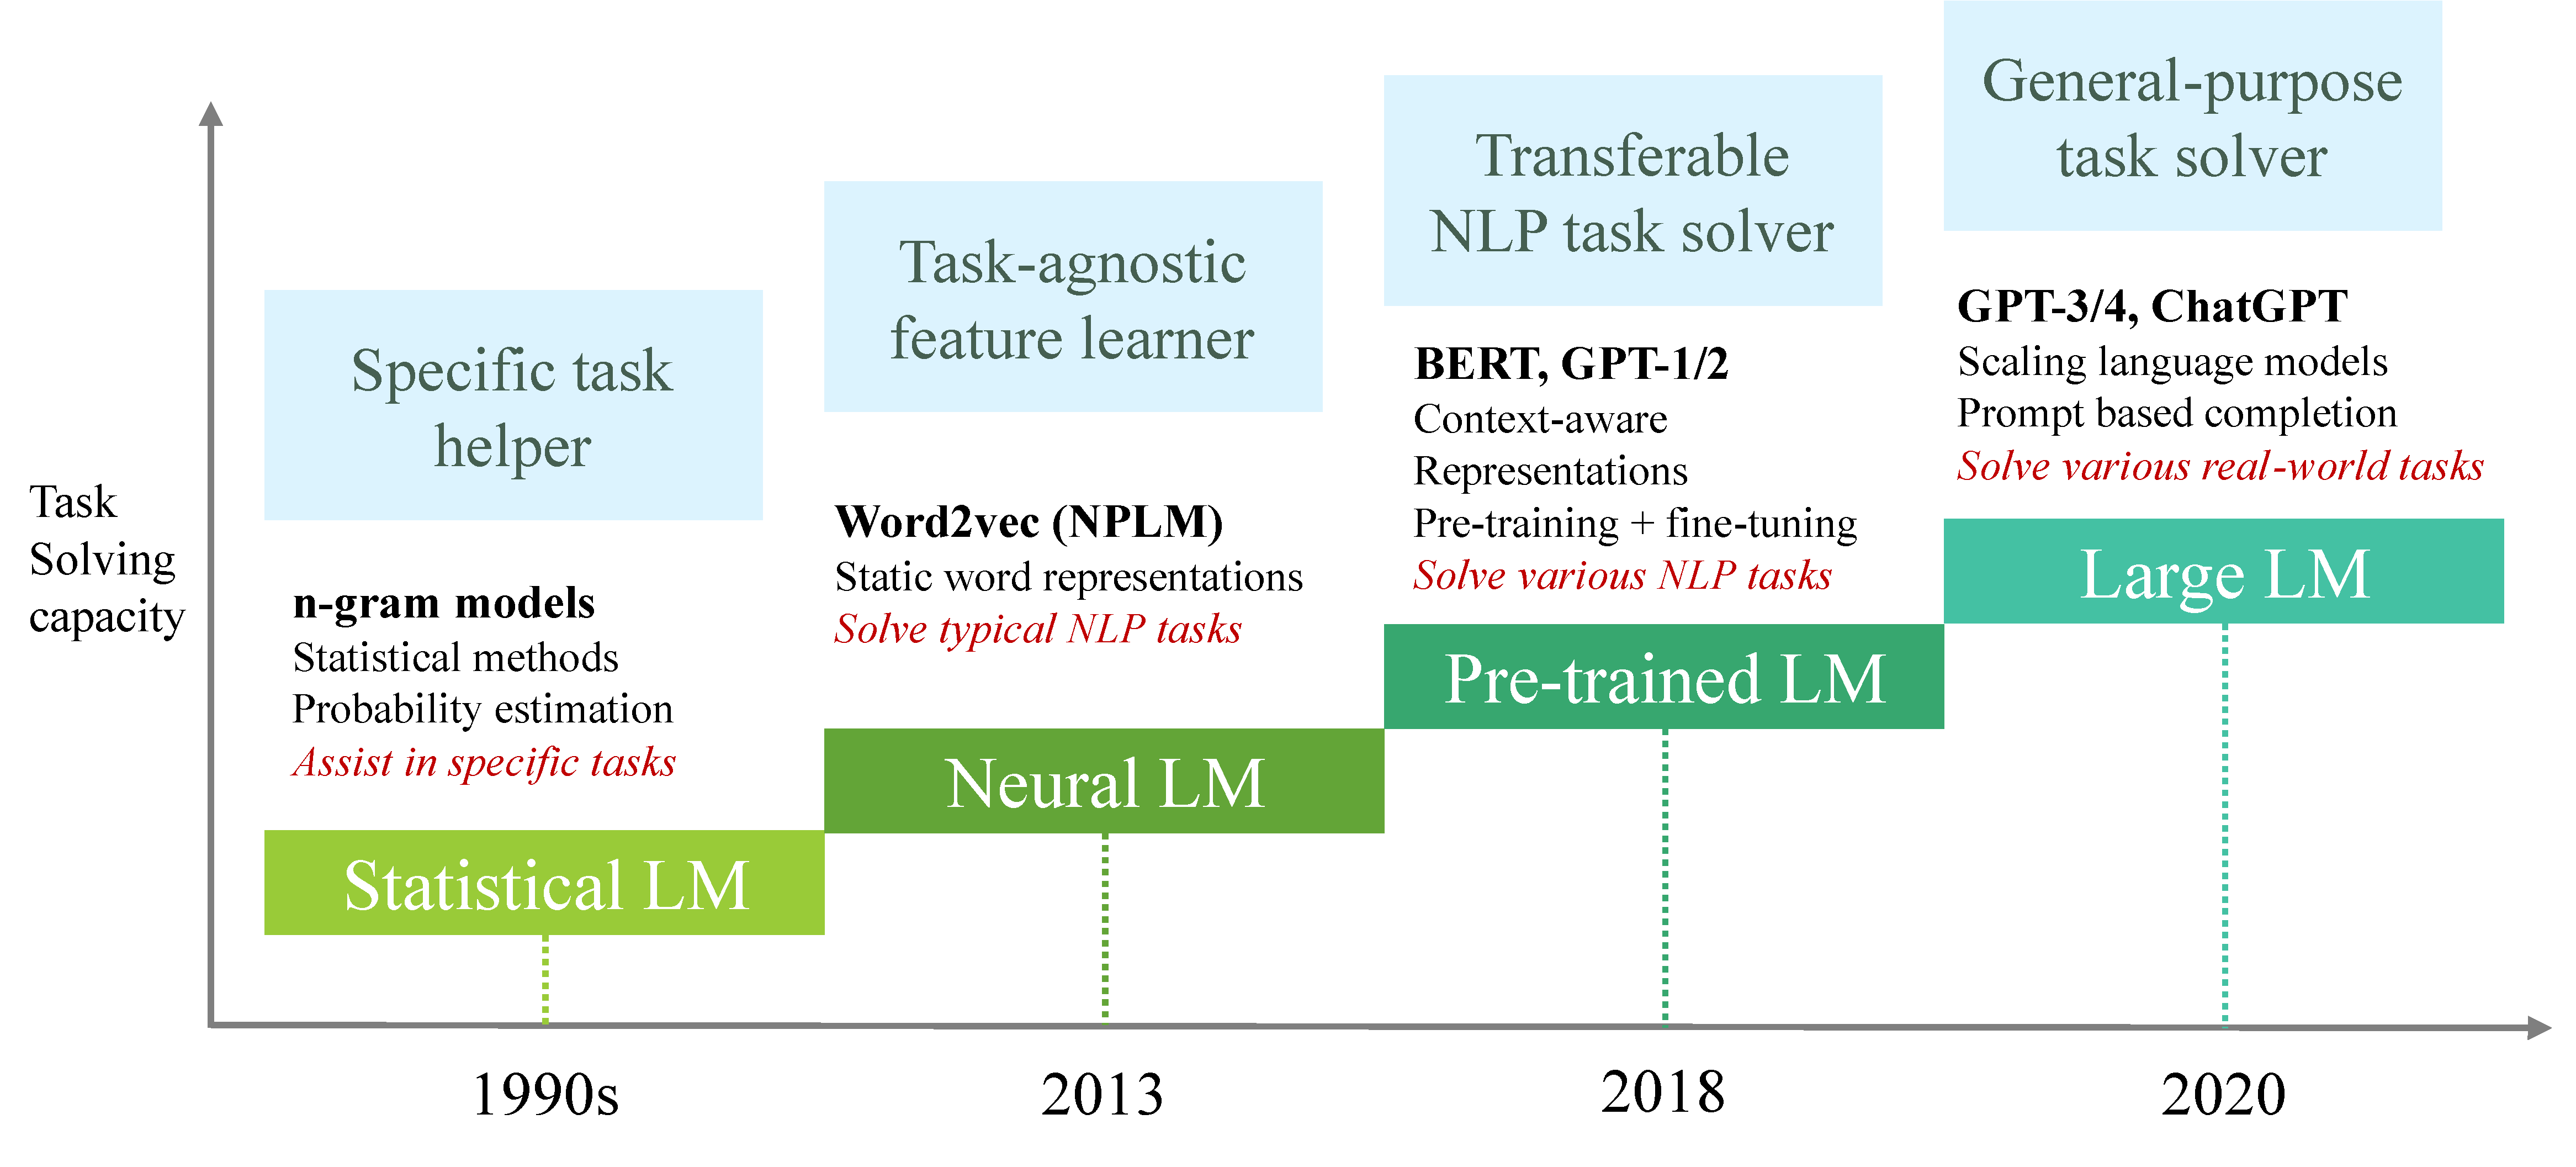
\includegraphics[width=\linewidth]{images/languagemodels}
    \caption[TODO.]{TODO~\autocite{zhao2023survey}}
    \label{fig:language-models}
\end{figure}

%With the introduction of the transformer architecture in 2017~\autocite{vaswani2023attention}
%task-agnostic representations -> less human feature engineering~\autocite{zhao2023survey}

%from~\autocite{zhao2023survey}:
%language modeling to task solving

%from ~\autocite{Raiaan2024ARO}:
%pre-training on large corpora from the web -> learning complicated patterns and language subtleties
%fine-tuning on downstream tasks gives state-of-the-art performance
%"comprehend, produce, forecast human language"

%From ~\autocite{Hadi_2023}:
%during pre-training: models see diverse texts and learn grammar, facts, reasoning

\clearpage


\section{Deep Learning}\label{sec:deep-learning}
As previously mentioned, \glspl{dnn} are the underlying technology for modern language models.
\glspl{dnn} belong to the field \enquote{Deep Learning} which is a specific type of \gls{ml}.
The term \acrlong{ml} describes different computational methods that can learn to perform different tasks from experiencing data~\autocite{Goodfellow-et-al-2016}.

A typical application for \gls{ml} is to learn a task that can be represented by a mapping:
\[
    f: \mathcal{X} \rightarrow \mathcal{Y}
\]
The \textit{input space} $\mathcal{X}$ is the set of all possible \textit{examples}.
Each example is mapped to a \textit{label} or \textit{target value} from the \textit{target space} $\mathcal{Y}$.
Input spaces often consist of real vectors $\boldsymbol{x} \in \mathbb{R}^n$.
The entries $x_i$ of an example vector are called \textit{features}.
Target spaces vary depending on the specific task.
Typical are subsets of natural numbers for \textit{classifications} or real numbers (e.g.\ for \textit{regression}).

For classification tasks, the learned function assigns an integer representing a category to each possible input example.
A common use case for this is the categorization of images.
An automatic image classifier $f:\mathbb{R}^n \rightarrow \{1,\dots,k\}$ receives an image (usually in the form of a real vector) and outputs a numerical value that symbolizes the content of that image e.g.\ a person, an object or an animal.

\gls{ml} offers a broad range of methods to find functions that can model complex behavior.
They incorporate many elements from different fields like linear algebra, probability theory, numerical optimization and information theory~\autocite{Goodfellow-et-al-2016}.
\gls{ml} has been successfully applied to numerous problems from different domains, including text classification, \gls{nlp}, speech processing applications, computer vision and computational biology applications.
\gls{ml}-approaches are usually categorized into the different learning scenarios \textit{supervised learning}, \textit{unsupervised learning} and \textit{semi-supervised learning}.
These scenarios differ in the usage and type of available training data~\autocite{mohri2018foundations}.
Supervised learning is especially relevant for machine translation tasks like \gls{ats}.

\subsection{Supervised Learning}\label{subsec:supervised-learning}
In the setting of supervised learning, available training data consists of pairs of input examples with corresponding target values.
\[
    D = \{(x_1, y_1), \dots, (x_m, y_m)\}
\]
The general aim is to model the relation between the examples $x_i$ and the targets $y_i$.
For that, assumptions about the origin of the data have to be made.
It is commonly assumed that the pairs $(x_i, y_i)$ are sampled from an unknown probability distribution, i.e.\ they are realizations of random variables $Z_i = (X_i, Y_i)$ that take values in $\mathcal{X} \times \mathcal{Y}$.
The random variables $\{(X_1, Y_1), \dots ,(X_m, Y_m)\}$ are independently and identically distributed (i.i.d.) while $X_i$ and $Y_i$ are not necessarily independent~\autocite{gressmann2019probabilistic}.
In the context of \gls{ml} this is often denoted as $(X_i,Y_i) \sim P(X, Y)$ where $P(X, Y)$ signifies the joint probability distribution (e.g.\ \textcite{Goodfellow-et-al-2016}).

In the setting of \enquote{classical} supervised learning, the objective is to learn a deterministic prediction function $f: \mathcal{X} \rightarrow \mathcal{Y}$ that defines a mapping between examples and targets:
\[
    \, (X^*, Y^*) \sim P(X, Y): \quad  Y^* = f(X^*)
\]
To approximate this mapping, a set of potential prediction functions $\mathcal{H}$ is considered.
% TODO example
The learning algorithm consists of choosing the hypothesis $h \in \mathcal{H}$ that is closest to the unknown prediction function $f$, i.e.\ $h(X^*) \approx f(X^*) = Y^*$.
In order to quantify the mathematical distance between predictions, a \textit{loss function} (sometimes called \textit{cost function} or \textit{error function}) $L: \mathcal{Y} \times \mathcal{Y} \rightarrow \mathbb{R}$ is used.
If $\mathcal{Y} = \mathbb{R}$ (e.g.\ for a regression) the \textit{least squares loss} $L_{sq} (\hat{y}, y) = (\hat{y} - y)^2$ is common~\autocite{gressmann2019probabilistic}.
The ideal hypothesis $h^*$ minimizes the expected generalization error (sometimes called \textit{risk})
\[
    h^* = \underset{{h \in \mathcal{H}}}{\operatorname{argmin}} \, \mathbb{E}[L(h(X^*), Y^*)]
\]
Because the underlying data distribution $P(X, Y)$ is unknown, this optimization problem is not solvable.
Instead, the observed training data $D$ is used to minimize an approximation of the risk, i.e\ the \textit{empirical risk}:
\[
    \hat{h} = \underset{{h \in \mathcal{H}}}{\operatorname{argmin}} \, \frac{1}{m}\sum_{i=1}^{m} L(h(x_i), y_i)
\]
This approach may lead to \textit{overfitting}, meaning the determined hypothesis $\hat{h}$ accurately describes the training data $D$ but does not generalize well on unseen data.
There are several methods to prevent this like regulating the complexity and capacity of functions included in $\mathcal{H}$ or using a larger dataset with more training examples.
By setting aside a small subset of the training data as \textit{test data} which is not used in the optimization process, it is possible to estimate the generalization error.
This is again done with the empirical quantity specified above.
The estimate indicates how well the chosen hypothesis $\hat{h}$ performs on unseen data.

While learning a direct mapping from $\mathcal{X}$ to $\mathcal{Y}$ can be adequate to model some tasks, many supervised learning algorithms estimate a conditional probability distribution $P(Y | X)$ instead.
This way, the model can consider the \textit{aspect of uncertainty} that is present in many real world applications for \gls{ml}.
In this scenario, the desired prediction function maps input examples to a distribution over the target space $f: \mathcal{X} \rightarrow \operatorname{Distr}(\mathcal{Y})$.
To evaluate predictions, an appropriate loss function $L: \operatorname{Distr}(\mathcal{Y}) \times \mathcal{Y} \rightarrow \mathbb{R}$ is necessary.
For a classification task, the output distribution could be a categorical distribution over all class labels, i.e.\ a discrete distribution that for a given example $x$ assigns each class a probability signifying a degree of belief~\autocite{Goodfellow-et-al-2016}.
This type of prediction function can easily be modified to mimic the behavior of the \enquote{classical} prediction function:
\[
    g(x) =\underset{y \in \mathcal{Y}}{\operatorname{argmax}} [f(x)](y) \approx \underset{y \in \mathcal{Y}}{\operatorname{argmax}} P(Y=y|X=x)
\]

\subsection{Learning from Data (Gradient Descent)}\label{subsec:learning-from-data}
Depending on the type of assumed hypothesis functions, different methods from the field of \enquote{mathematical optimization} can be used to minimize the empirical risk.
It is typical to consider a set of functions $\{h(\,\cdot\, ; \boldsymbol{\theta}) \mid \boldsymbol{\theta} \in \Theta \}$ as the hypothesis space $\mathcal{H}$ where $\boldsymbol{\theta}$ represents free, learnable parameters that can be adjusted so the prediction function $h$ can accurately fit the data $D$.
The parameter space $\Theta$ is often chosen as $\mathbb{R}^n$ meaning the function is parameterized by a vector of real numbers.
A simple example for such a set of functions is the linear combination $h(\boldsymbol{x}, \boldsymbol{\theta}) = x_1\theta_1 + \dots + x_n\theta_n$.

The empirical risk can then be formulated as a function $\mathcal{L}: \Theta \rightarrow \mathbb{R}$:
\[
    \mathcal{L}(\boldsymbol{\theta}) = \frac{1}{m}\sum_{i=1}^{m} L(h(x_i, \boldsymbol{\theta}), y_i)
\]
Finding the hypothesis $\hat{h}$ that most accurately describes the training data can now be solved by minimizing $\mathcal{L}(\boldsymbol{\theta})$ with respect to \boldsymbol{\theta}.
Assuming that \boldsymbol{\theta} is a vector, a minimum needs to satisfy the condition of stationary ($\nabla$ referring to the gradient i.e.\ a vector of partial derivatives)
\[
    [\nabla\mathcal{L}](\boldsymbol{\theta}) = 0
\]
For very complex hypothesis functions, this is usually not directly solvable.
Moreover, to guarantee that a stationary point is indeed a minimum and not a maximum or saddle point, additional conditions need to be met.
Iterative solvers mitigate some of the aforementioned issues and are thus a popular solution for this kind of optimization problem.

The gradient $[\nabla\mathcal{L}](\boldsymbol{\theta})$ describes how the value of the function $\mathcal{L}$ reacts to slight changes in the input $\boldsymbol{\theta}$.
Evaluating the gradient in any point $\boldsymbol{\theta} \in \Theta$ returns a vector in the parameter space $\Theta$ that points in the direction that results in the steepest ascent in the value of $\mathcal{L}$.
Likewise, the opposite direction of that vector aligns with the direction of the steepest descent.
With this intuition, it becomes obvious that for small enough $\epsilon$ the following inequality holds:
\[
    \mathcal{L}(\boldsymbol{\theta}) > \mathcal{L}(\boldsymbol{\theta} - \epsilon\,[\nabla\mathcal{L}](\boldsymbol{\theta}))
\]
Hence, taking small steps in the direction of the negative gradient should eventually lead to a local minimum.
This motivates the iterative method called \enquote{gradient descent} or \enquote{steepest descent}.
After randomly initializing $\boldsymbol{\theta_0}$ (preferably close to zero) the following update is iteratively calculated:
\[
    \boldsymbol{\theta_{t+1}} = \boldsymbol{\theta_{t}} + \epsilon\,[\nabla\mathcal{L}](\boldsymbol{\theta_{t}})
\]
The variable $\epsilon$ is called the \textit{learning rate}.
It controls the magnitude of each update and is usually chosen to be a real number close to zero (e.g.\ 0.01). % TODO: source
The learning rate does not have to be a fixed value.
It can also be adaptively determined in each step, e.g.\ by optimizing for $\epsilon$ to find the step size that results in the greatest decrease in $\mathcal{L}$.
This method is known as \enquote{line search}.

The gradient descent algorithm terminates when all elements of the gradient are equal or close to zero.
The final value $\boldsymbol{\hat{\theta}}$ for $\boldsymbol{\theta_{i}}$ is an approximate solution to the optimization problem and can be used as the parameter for the final prediction function $\hat{h}(\,\cdot\,; \boldsymbol{\hat{\theta}})$.

A necessary prerequisite for gradient descent is that the empirical error function is differentiable.
This strongly depends on what kind of hypothesis functions are considered.
Moreover, for non-convex functions convergence of the algorithm is not guaranteed.
In theory, gradient descent can converge in saddle points or undesirable local minima, as in these critical points the gradient will be close to zero.
However, in practice, the method has proven to reliably find low values in the error function in reasonable time.
Gradient methods are usually not attracted to maxima and rarely get stuck in saddle points.
Although they almost never terminate in the global minimum, a sufficiently small local minimum can be determined more often than not.

There is a large variety of modified gradient descent methods that can stabilize or accelerate the training procedure.
Examples for this are methods that use the gradients of several previous steps to calculate the update (e.g.\ \enquote{gradient accummulation}, \enquote{Nesterov} or \enquote{momentum}) and methods that use second derivatives (e.g.\ \enquote{Newton methods}).

A very popular variation in deep learning is \gls{sgd}.
Computing the exact gradient is slow, as it can be composed of millions of training examples.
Increasingly large datasets lead to more expensive calculations.
\gls{sgd} takes advantage of the fact that in the setting of supervised learning, the empirical error function is often composed of point-wise loss functions.
By only calculating the loss on a subset $B \subset \{1,\dots,m\}$ of the training data $D$, computation cost can be greatly reduced.
\[
    \hat{\mathcal{L}}(\boldsymbol{\theta}) = \frac{1}{|B|}\sum_{i \in B} L(h(x_i, \boldsymbol{\theta}), y_i)
\]
The \textit{minibatches} $B$ are sampled randomly.
As long as no examples are repeated, the gradient of the partial empirical error $\hat{\mathcal{L}}(\boldsymbol{\theta})$ is an unbiased estimate of the true generalization error's gradient.
Furthermore, usage of small minibatch sizes can have a regularization effect.
This makes overfitting less likely.
While \gls{sgd} progresses fast in the early training phase, convergence is generally slower than for standard gradient descent.
But because this faster convergence does not correspond with a faster decrease in the generalization error, \gls{sgd} with all its benefits is usually the preferred algorithm.
For optimal convergence conditions, the learning rate for \gls{sgd} needs to be gradually decreased~\autocite{Goodfellow-et-al-2016}.

\subsection{Neural Networks}\label{subsec:dnn}
An important part of solving tasks with \gls{ml} is the choice of the hypothesis space $\mathcal{H}$.
Considering functions with a very high capacity (i.e.\ complex functions with many free parameters) might lead to overfitting.
Choosing a very simple family of functions to model the task might not suffice to accurately represent it.
Usually, the capacity needs to be in line with the complexity of the target task for \gls{ml} algorithms to perform best~\autocite{Goodfellow-et-al-2016}.

In deep learning, \textit{neural networks} are used as hypothesis functions.
Neural networks are mathematical functions that are composed of many simpler functions~\autocite{Goodfellow-et-al-2016}.
While the term \enquote{deep learning} is still quite new, the first approaches for neural networks can be traced back to the 1940s.
These early neural networks were motivated by the idea to model the human brain and explored if it was possible for a mathematical function to learn intelligent behaviour.
In this context, neural networks are referred to as \glspl{ann}.
However, in neuroscience, neural networks are not considered a realistic model of the human brain.

The earliest models were based on simple linear or affine functions that take a vector $\boldsymbol{x}$ of length $n$ as an input and map them to a single output $y$~\autocite{Goodfellow-et-al-2016}.
The learnable parameters $\boldsymbol{\theta} = (\boldsymbol{w}, b)$ are a vector $\boldsymbol{w}$ of \textit{weights} and a \textit{bias}\footnote{not refering to the statistical bias} term $b$.
\[
    f(\boldsymbol{x}; \boldsymbol{\theta}) = f(\boldsymbol{x}; \boldsymbol{w}, b) = x_1 w_1 + \dots + x_n w_n + b
\]
Such a model can, among other things, be used for binary classification.
When setting $f(\boldsymbol{x}; \boldsymbol{w}, b)$ equal to zero, the equation defines a hyperplane in the input space $\mathcal{X}$ where $\boldsymbol{w}$ is the normal vector of that plane.
The hyperplane divides the input space in two regions.
Evaluating $f$ in $\bodsymbol{x}$, i.e.\ calculating the dot product with $\boldsymbol{w}$, projects the input onto the normal vector of the plane.
In the case of unit vectors, the absolute value of the dot product can be understood as the distance between $\boldsymbol{x}$ and the hyperplane.
The sign of $f(\boldsymbol{x}; \boldsymbol{w}, b)$ indicates on which side of the hyperplane the point $\boldsymbol{x}$ lies~\autocite{bishop2006}.

In a similar way, the earliest predecessors of neural networks like the \enquote{McCulloch-Pitts Neuron} in the 1940s and the \enquote{perceptron} in the 1950s could categorize inputs.
In the 1960s, major limitation of linear models led to a temporary decline of this method.
Specifically, it was found that the models could not learn the very simple \textit{XOR} (exclusive or) function that takes two binary inputs and maps them to a single binary output as follows:
\[
    f([0,0]; \boldsymbol{\theta}) = 0, \quad
    f([0,1]; \boldsymbol{\theta}) = 1, \quad
    f([1,0]; \boldsymbol{\theta}) = 1, \quad
    f([1,1]; \boldsymbol{\theta}) = 0
\]
\begin{figure}
    \centering
    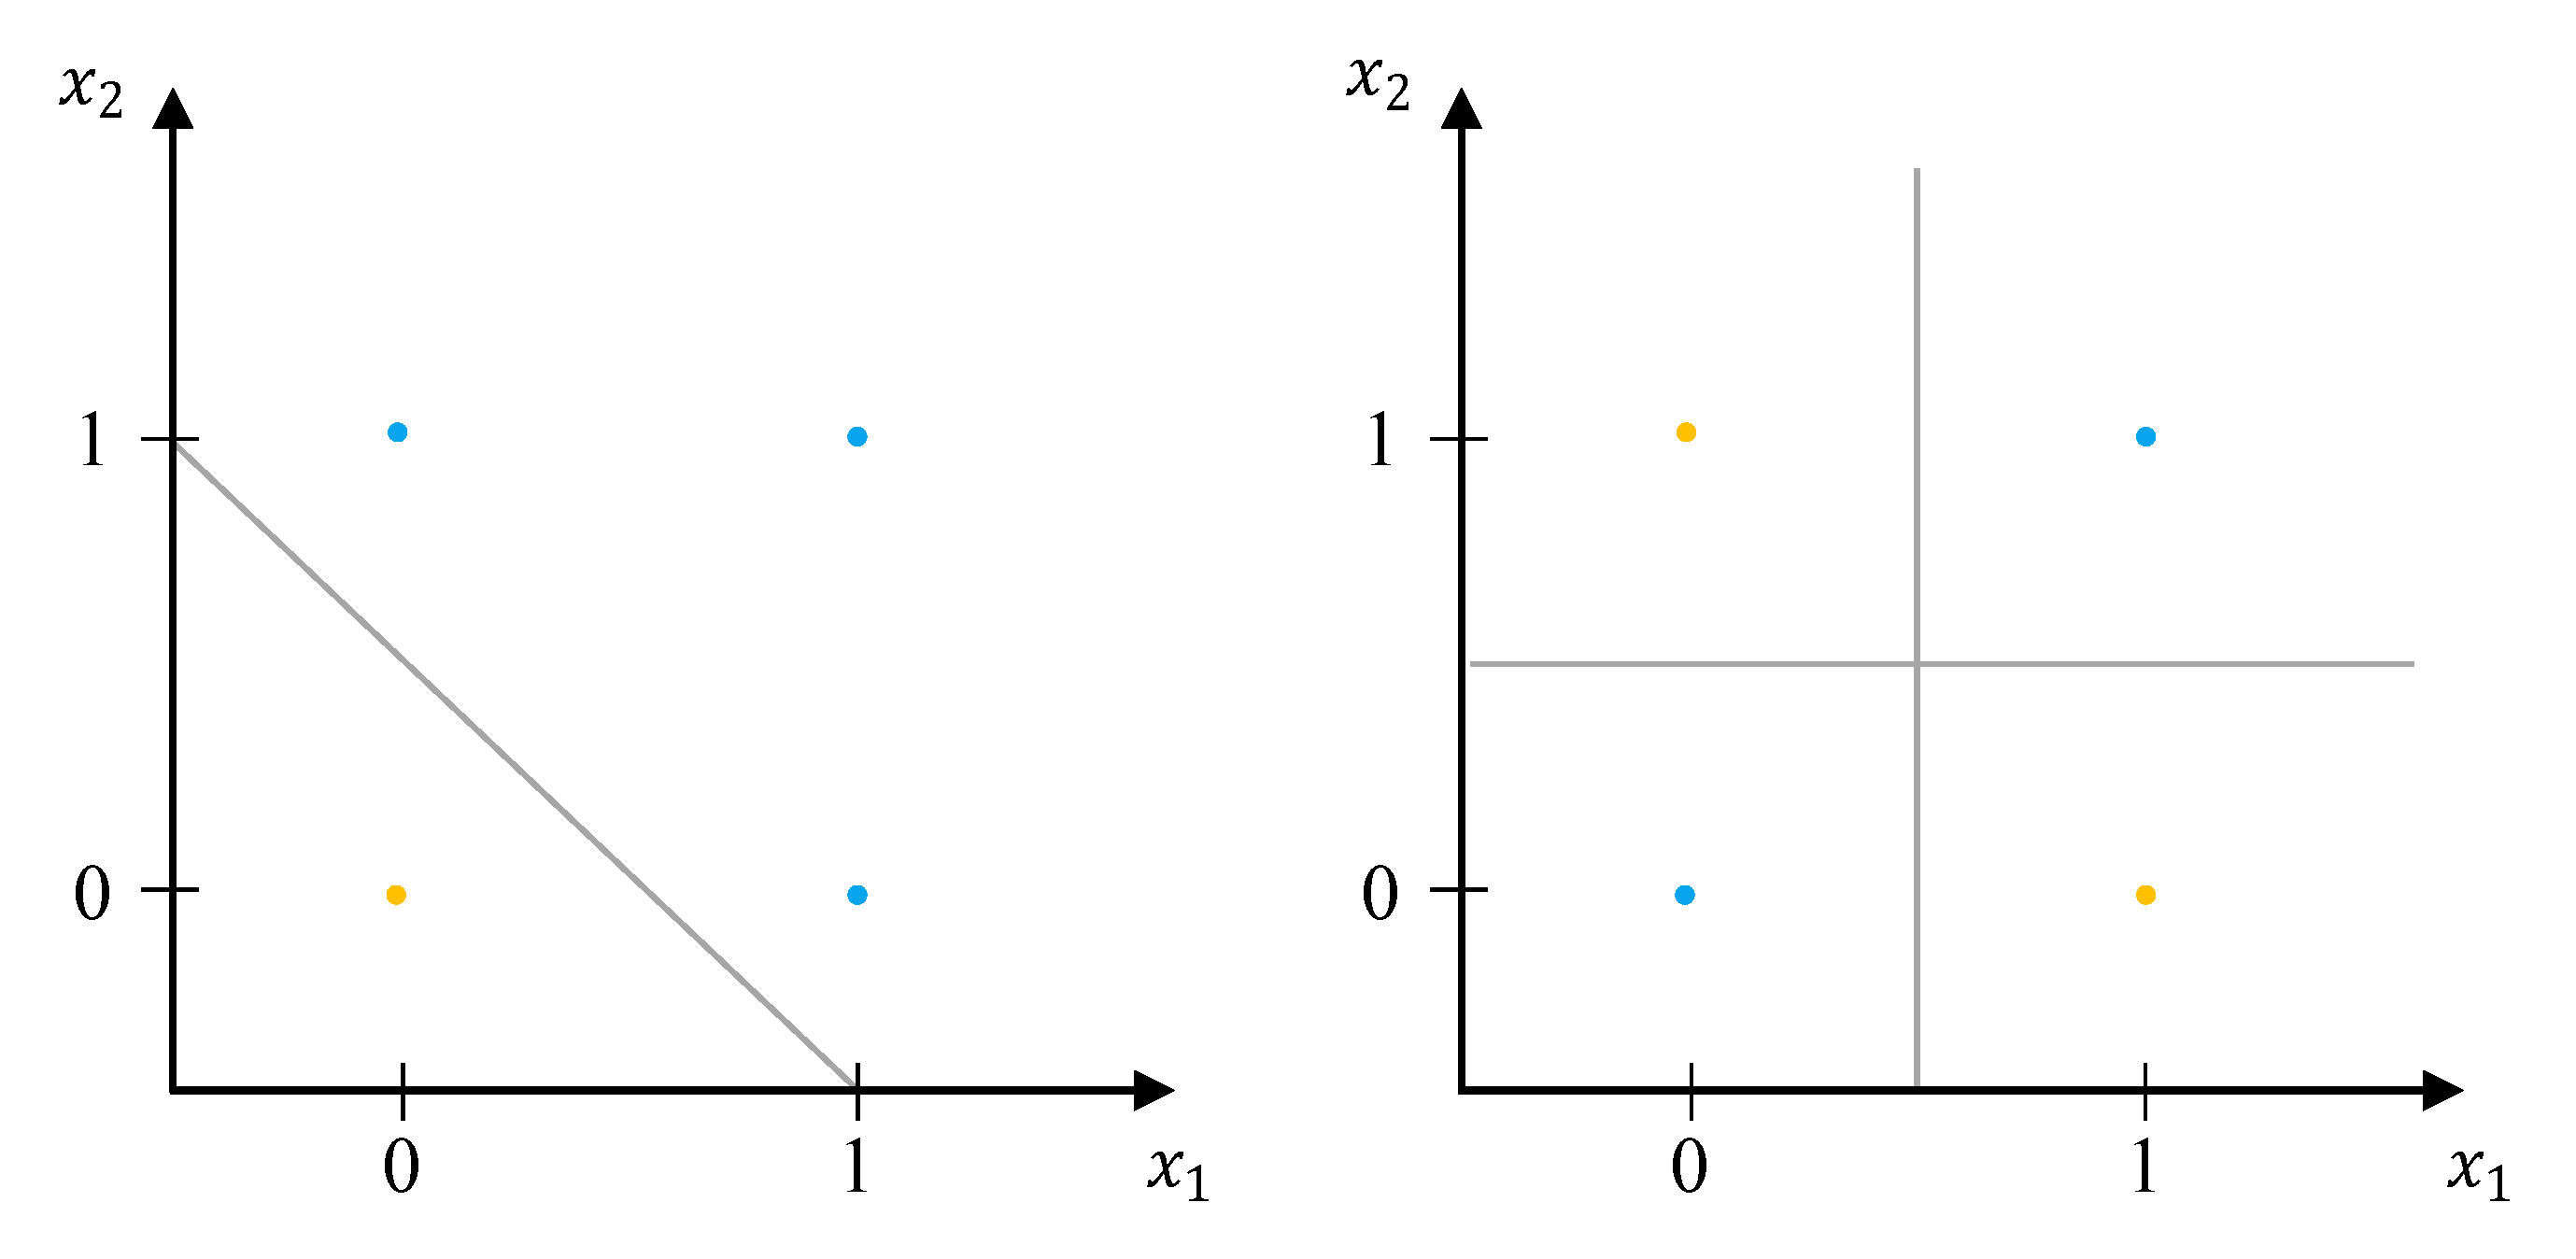
\includegraphics[width=.9\linewidth]{images/xor}
    \caption[Limits of the linear model.]{While linear models can learn decision boundaries for \textit{linear separable} data, e.g.\ learning the \textit{logical or}-function (left), they are incapable of learning non-linear decision boundaries, e.g.\ the \textit{XOR}-function (right)~\autocite{sonnet2022NeuralBoook}.}
    \label{fig:xor}
\end{figure}
As seen in \autoref{fig:xor}, linear models can only learn linear \textit{decision boundaries}.

In the 1980s, the movement of \enquote{connectionism} improved upon these initial approaches.
The main idea of this movement is that a large number of simple computational units (i.e.\ neurons) can realize intelligent behaviour when working together.
With this idea in mind, a possible solution for the XOR-problem is given by feeding the input in two independent linear models and combining their outputs in a third linear model.

More precisely, the inputs $\boldsymbol{x} = [x_1,x_2]$ are initially mapped to an intermediate state often referred to as \enquote{hidden units}.
\begin{align*}
    f^{(1)}(\boldsymbol{x}; \boldsymbol{w_1}, b_1) = g(\boldsymbol{w_1}^T \boldsymbol{x} + b_{1}) = z_1 \\
    f^{(2)}(\boldsymbol{x}; \boldsymbol{w_2}, b_2) = g(\boldsymbol{w_2}^T \boldsymbol{x} + b_{2}) = z_2
\end{align*}
Because the composition of multiple linear functions would just collapse into another linear function, a non-linear \textit{activation function} $g$ is applied.
A function that is commonly used is the \textit{rectified linear unit} or \textit{ReLU} defined as $g(v) = \max\{0, v\}$.
The hidden units are then passed to the third linear model which produces the final output:
\[
    f^{(3)}(\boldsymbol{z} = [z_1, z_2]; \boldsymbol{w_3}, b_3) = \boldsymbol{w_3}^T \boldsymbol{z} + b_{3} = y
\]
The function $f^{(1)}$ and $f^{(2)}$ can be combined into a single function $f^{\{1, 2\}}$ parameterized by a weight matrix $\boldsymbol{W}$ and a bias vector $\boldsymbol{b}$:
\[
    f^{\{1, 2\}}(\boldsymbol{x}; \boldsymbol{W}, \boldsymbol{b}) = g(\boldsymbol{W}^T \boldsymbol{x}+ \boldsymbol{b}) = \boldsymbol{z} \\
\]
The non-linear function $g$ is applied component wise.
The complete network can now be written as a simple composition of functions:
\[
    f(\boldsymbol{x}) = f^{(3)}(f^{\{1, 2\}}(\boldsymbol{x}))
\]
$f^{(1)}$, $f^{(2)}$ and $f^{(3)}$ are called the \enquote{neurons} of the network.
Multiple neurons that can be computed in parallel are called a layer.
In this case $f^{\{1, 2\}}$ is called a \enquote{hidden layer}, the inputs $\boldsymbol{x}$ are the \enquote{input layer} and $y$ is the \enquote{output layer}.

With this simple neural network, it is indeed possible to learn the XOR-function.
Furthermore, this method can be modified to find functions that can approximate almost any possible function.
The \textit{universal approximation theorem} states, that a network with a linear output layer and a hidden layer with an appropriate non-linear activation function can represent any Borel measurable function that maps from one finite-dimensional space to another, as long as there are enough hidden units~\autocite{Goodfellow-et-al-2016}.
In practice, it is not feasible to use such a single layer network because the number of necessary hidden units grows exponentially for more complex functions.
Instead, it is common to add more hidden layers by chaining more functions:
\[
    f(\boldsymbol{x}) = f^{(4)}(f^{(3)}(f^{(2)}(f^{(1)}(\boldsymbol{x}))))
\]
The number of hidden layers is called the \enquote{depth} of the network.
The depth is also what the term \enquote{deep learning} refers to.
It is not exactly defined what number of layers a neural network needs to be called \textit{deep}.
But a \acrlong{dnn} can be generally understood as a neural network with many layers.

The previously described neural network is known as a \enquote{feedforward neural network} or \gls{mlp}.
It can be easily scaled by adding any number of layers with any number of neurons.
A typical way of visualizing a \gls{mlp} can be seen in \autoref{fig:neural-network}.
\begin{figure}
    \centering
    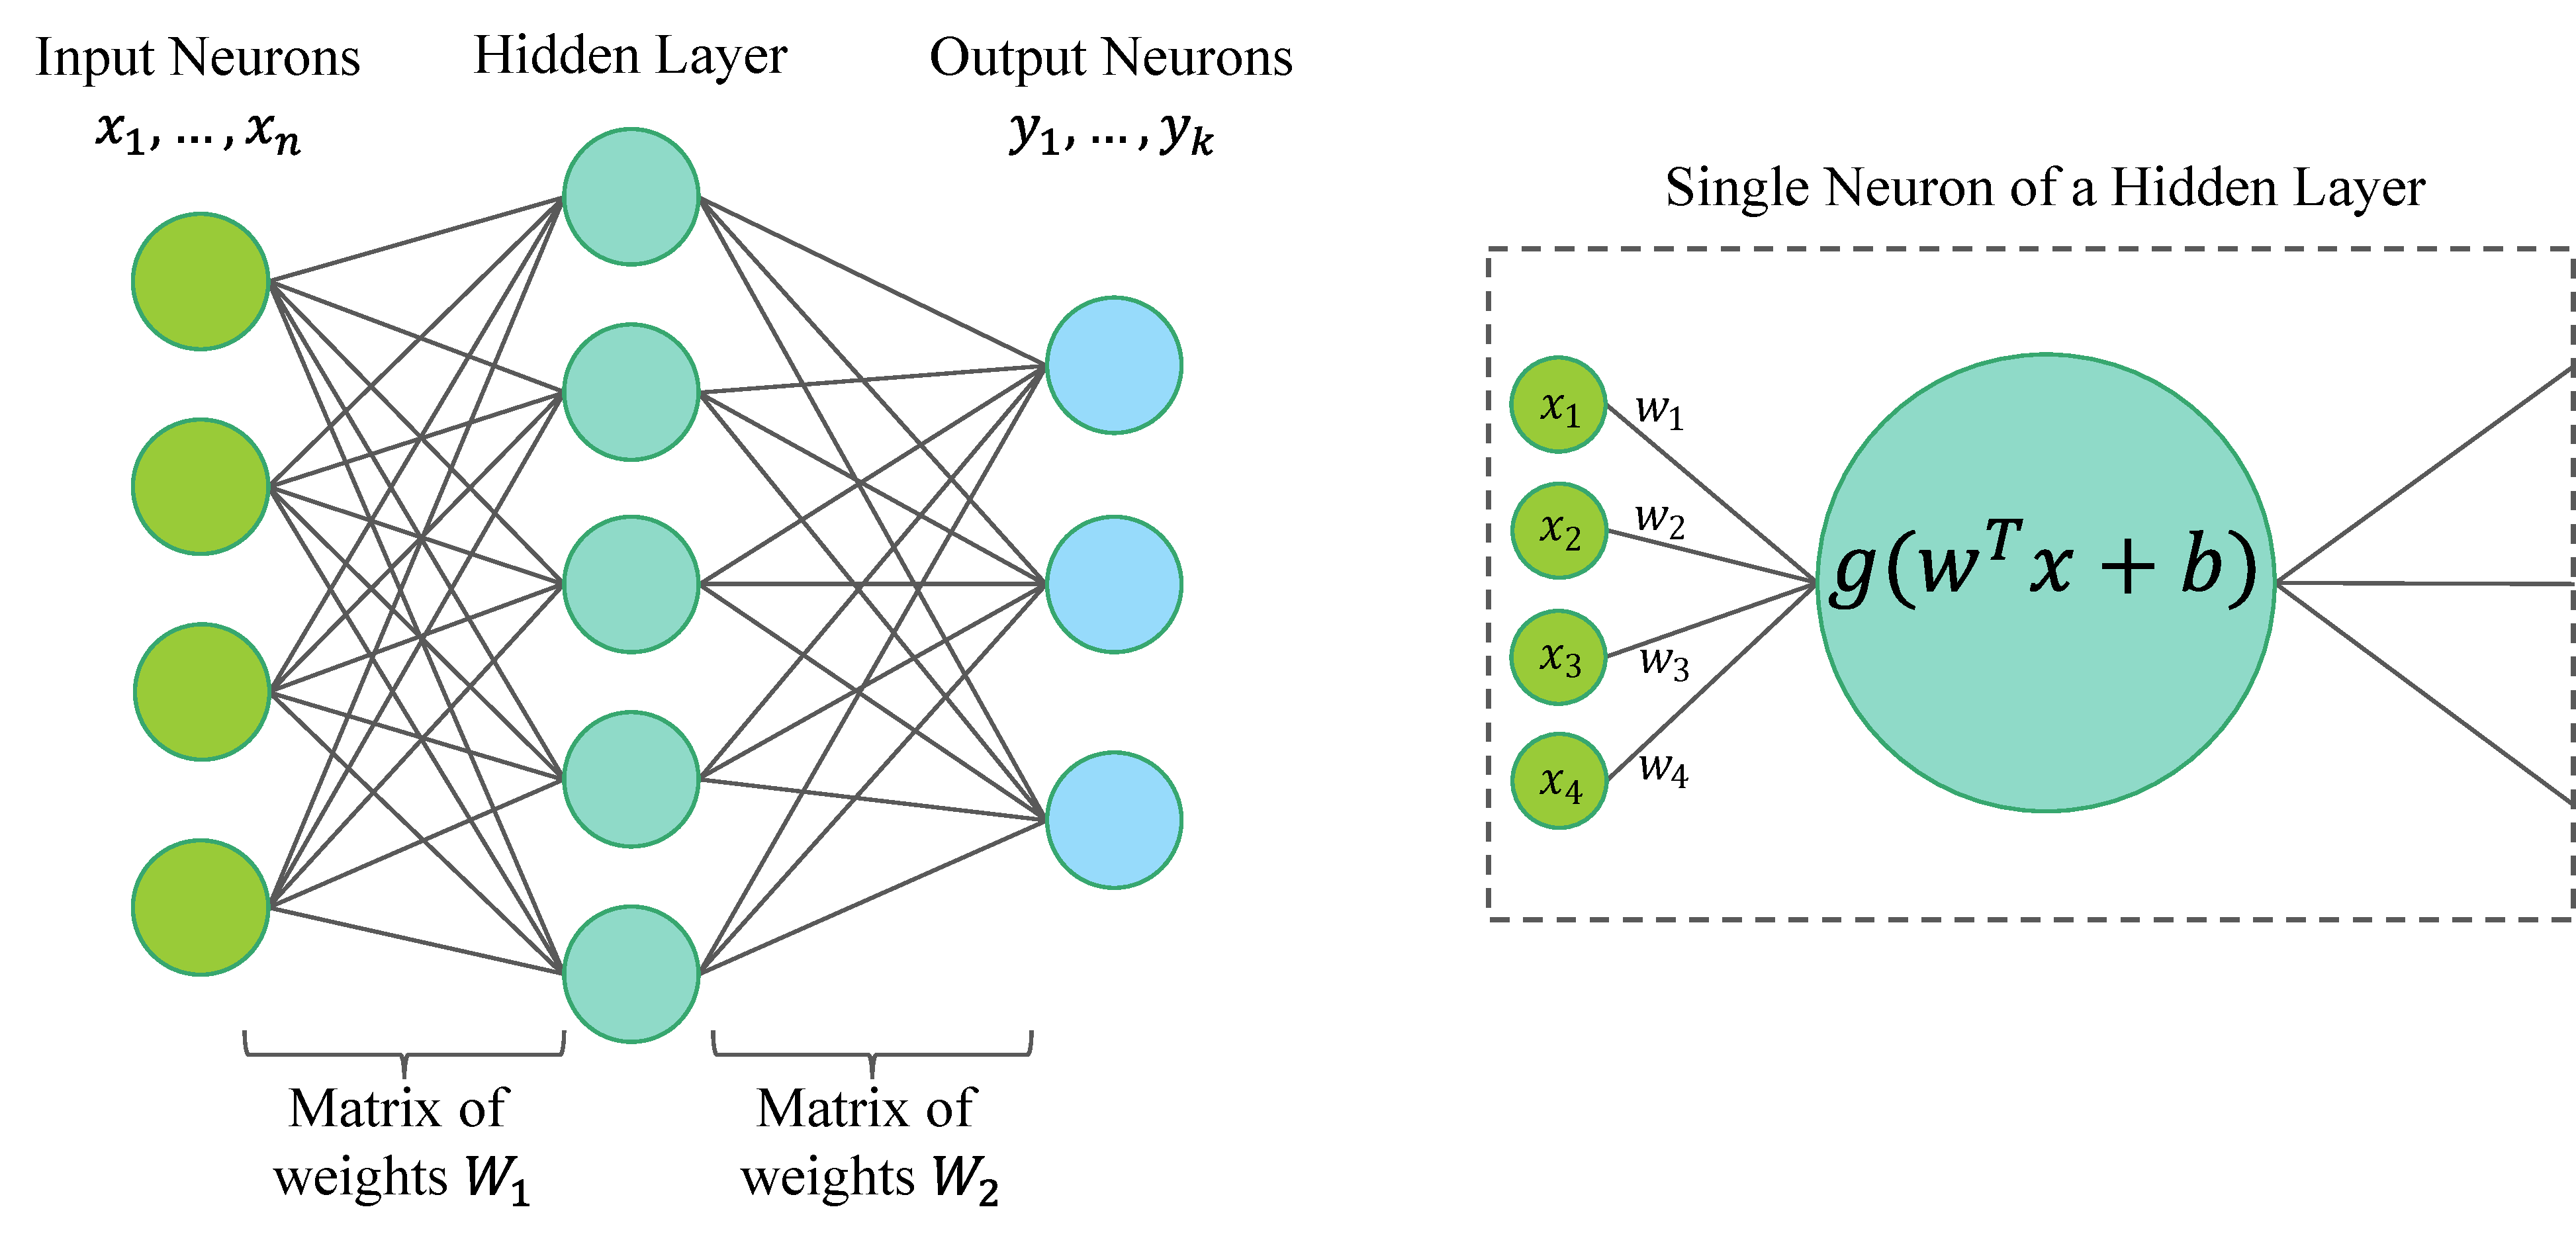
\includegraphics[width=\linewidth]{images/nn}
    \caption[Visualization of a neural network.]{Neural networks are often visualized as directed graphs. This \gls{mlp} (left) has four input neurons, one hidden layer with five neurons and three output neurons. Each hidden unit or neuron is represented by a node. The edges between neurons stand for the weights that are applied to the incoming signals. The edges between two layers are mathematically described by a single matrix $\boldsymbol{W}$ that multiplied with the previous outputs gives the inputs for the next layer~\autocite{sonnet2022NeuralBoook, Goodfellow-et-al-2016}.}
    \label{fig:neural-network}
\end{figure}
% \enquote{feedforward} because information flows only in one direction

\glspl{dnn} like the \gls{mlp} have been successfully applied to many tasks like \textit{speech recognition}, \textit{image segmentation} and \textit{optical character recognition}.
They incorporate little task-specific assumptions and are thus a very general approach.
The design of \glspl{mlp} makes it possible to choose input and output dimensions freely to describe any supervised learning task.
\glspl{mlp} handle high dimensional data (e.g.\ images) well.
This is related to the ability of \glspl{dnn} to learn features automatically from raw input data.
In traditional \gls{ml}-applications the features that were passed to the model as inputs were often selected by hand.
The raw input data was processed, so only information relevant to the task remained.
This is known as \textit{Feature Engineering}.
Depending on the complexity of the task and data, a lot of manual effort is needed to find effective features.
Having the model learn the features automatically is called \enquote{feature learning} or \enquote{representation learning}.

The concept of \textit{representations} is crucial to deep learning.
\glspl{mlp} generate a new representation of the input at each layer.
During supervised training, earlier layers learn to output representations that make the target task easier.
Looking back at the XOR-function (\autoref{fig:xor}), the input data is initially not linear separable which changes after it is passed through the first layer.
The hidden layer maps the inputs into a different feature space, where the classification task is easier.

An intuition for \glspl{dnn} is that specific layers learn different concepts, i.e.\ they output representations that carry information about that concept.
This motivates the reuse of certain parts of the network which is known as \enquote{transfer learning}.
Building networks that can find expressive, general purpose representations for input data has been a central object of research.
In the domain of language, representations for words (i.e.\ embeddings) are especially important as inputs in natural language initially do not lie in a vector space~\autocite{Goodfellow-et-al-2016}.
\glspl{dnn} have been successfully used to create powerful word representations that generalize well for many different tasks~\autocite{zhao2023survey}.
% TODO: connection to language model introduction

%often better than hand selected features

%factors of variation make learning difficult (e.g. recognizing a car in an image -> different angles)
%more available data -> Deep Learning more useful
%overfitting no issue

%nesting of concepts in layers of network

%concept of distributed representation:
%3 subjects, 3 colors -> model should recognize all 9 combinations
%possible with 9 neurons that each learn to identify one combination
%better: 3 neurons describe color and 3 the type of object (concatenation? intermediate representation)

\subsubsection{Training for Neural Networks}
Neural networks are usually trained by applying some form of gradient descent.
Hence, the hypothesis function that is included in the loss needs to be differentiable.
Determining and evaluating the gradient for neural networks can be challenging and computational expensive as the networks may be composed of hundreds of layers and millions of parameters.

In order to update the parameter vector $\boldsymbol{\theta_t}$ in a single step of the optimization procedure, the gradients of the point-wise loss functions need to be evaluated in  $\boldsymbol{\theta_t}$:
\[
    [\nabla_{\boldsymbol{\theta}}  L(h(x_i, \boldsymbol{\theta}), y_i)](\boldsymbol{\theta_t})
\]
Input examples $x_i$, target values $y_i$ and predictions $\hat{y}_i = h(x_i, \boldsymbol{\theta})$ are fixed values.
If the hypothesis function $h$ is a \gls{mlp} with $l$ layers, the loss function is simply a composition of many functions.
\[
    \nabla_{\boldsymbol{W}, \boldsymbol{b}} \, L(g^{(l)}(\cdots g^{(2)}(W^{(2)}g^{(1)}(W^{(1)}x_i + b^{(1)}) + b^{(2)}) \cdots + b^{(l)}), y_i)
\]
Taking derivatives with regard to the learnable parameters $\boldsymbol{W, b}$ can be accomplished by applying the \textit{chain rule of calculus}.
Let $y = g(x)$ and $z = f(g(x)) = f(y)$.
The derivative of the composed function can be written as
\[
    \frac{dz}{dx} = \frac{dz}{dy}\frac{dy}{dx}
\]
Considering a simple \gls{mlp} similar to the one used in the XOR-problem, the intermediate steps in the \textit{forward computation} can be denoted as follows.
\[
    h(\boldsymbol{x}; \boldsymbol{W}, \boldsymbol{b}) =
    \overbrace{
        g^{(2)}\Biggl(
        \underbrace{
            \begin{pmatrix}
                w_{1}^{(2)} \\
                w_{2}^{(2)}
            \end{pmatrix}^{\top}
            \overbrace{
                g^{(1)} \Biggl(
                \underbrace{
                    \begin{pmatrix}
                        w_{11}^{(1)} & w_{12}^{(1)} \\
                        w_{21}^{(1)} & w_{22}^{(1)}
                    \end{pmatrix}
                    \begin{pmatrix}
                        x_1 \\
                        x_2
                    \end{pmatrix}
                    +
                    \begin{pmatrix}
                        b_1^{(1)} \\
                        b_2^{(1)}
                    \end{pmatrix}
                }_{z^{(1)}}
                \Biggr)
            }^{o^{(1)}}
            +
            \begin{pmatrix}
                b_1^{(2)} \\
                b_2^{(2)}
            \end{pmatrix}
        }_{z^{(2)}}
        \Biggr)
    }^{o^{(2)}}
\]
The partial derivative for a single weight of the last layer can be written as
\begin{align*}
    \frac{\partial L}{\partial w_1^{(2)}} &= \frac{\partial L}{\partial o^{(2)}} \frac{\partial o^{(2)}}{\partial z^{(2)}}  \frac{\partial z^{(2)}}{\partial w_1^{(2)}} \\
    &= \frac{\partial L}{\partial o^{(2)}} g^{(2)\prime} (z^{(2)}) o_1^{(1)}
\end{align*}
where $g^{(2)\prime}$ is the second derivative of the last activation function.
If the \textit{least squares loss} $L_{sq} (\hat{y}_i)= \frac{1}{2}(y_i - \hat{y}_i)^2$ with derivative $L_{sq}^{\prime} (\hat{y}_i) = (y_i - \hat{y}_i)$ is chosen, the term simplifies to
\begin{align*}
    \frac{\partial L}{\partial w_1^{(2)}} &= L_{sq}^{\prime} (o^{(2)}) g^{(2)\prime} (z^{(2)}) o_1^{(1)} \\
    &= (y_i - o^{(2)}) g^{(2)\prime} (z^{(2)}) o_1^{(1)}
\end{align*}
More generally, when regarding the neural network as a graph like in \autoref{fig:neural-network}, the partial derivative for a single weight can be calculated by forming it along the path from the last layer (respectively the loss function) to the edge that represents that weight.
For weights that are located further inside the network, multiple paths exist, which translates into multiple added terms that form the derivative.
Moreover, derivatives of later layers include terms that are needed to calculate derivatives of weights in the earlier layers.
This motivates the \textit{back-propagation} method that determines the gradient by recursively calculating the layer-wise derivatives from the back to the front of the network.
Before that, a forward propagation (i.e.\ calculating the loss for a training example) is necessary to gather the inputs and outputs of the activation functions that as seen above may appear in the partial derivatives.
Back-propagation avoids duplicate calculations by saving subexpression in memory, which reduces computational cost.

% not only for MLP but other neural networks
%\href{https://sudeepraja.github.io/Neural/}{A Derivation of Backpropagation in Matrix Form | Sudeep Raja}

% not analytical form of gradient is needed, but gradient evalutated in current parameter vector \theta

% Training dificult: inductive biases
% \enquote{incorporate doamin knowledge into the network} -> cnn, parameter sharing -> reduce trainable parameters while having equal size

% modern models designed  to have nice properties for optimization (LSTM) (seite 341)
% skip connection
% cnn: sprase interaction
% less calculations

%from~\autocite{sonnet2022NeuralBoook}:
%The term \enquote{Deep Learning} was first used in book in 2000

% MLPs have not been widely used in pratice: goodfellow and bias paper

%\subsubsection{Loss Functions / Example Classification}


\section{Transformers}\label{sec:trans}


\section{Decoder-only Models}\label{sec:decoder}

\subsection{GPT}\label{subsec:gpt}

\subsection{Llama}\label{subsec:llama}

\subsubsection{Leo}


\section{Supervised Fine-Tuning (SFT)}\label{sec:supervised-fine-tuning}


\section{Alignment Methods}\label{sec:alignment-methods}
from~\autocite{zhao2023survey}:
capture properties of training corpus

\subsection{RLHF}\label{subsec:rlhf}

\subsection{PPO}\label{subsec:ppo}

\subsection{DPO}\label{subsec:dpo}

    \chapter{Experiments}\label{ch:exp}


\section{Data Overview}\label{sec:data_ov}

\subsection{Plain Language and Easy Language Data}\label{subsec:plain-language-and-easy-language-data}


\section{Supervised Fine-Tuning}\label{sec:supervised-fine-tuning-exp}

\subsection{Architectures}\label{subsec:architectures}

\subsection{Synthetic Parallel}\label{subsec:synthetic-parallel}

% text is not reorganized -> very linear

\subsection{True Parallel}\label{subsec:true-parallel}

% Best model yet


\section{DPO Approach}\label{sec:dpo-approach}

\subsection{DPO-Data}\label{subsec:dpo-data}

\subsection{Annotation Process}\label{subsec:annotation-process}

\subsection{Problems}\label{subsec:problems}

% Computation Limmitation -> unsloth
% Bad annotation predictions -> Model not ready for DPO?
% Bad prediction on unseen domains


\section{Monolingual Pre-Training}\label{sec:monolingual-pre-training}

% Bad results


\section{Evaluation}\label{sec:evaluation}

% Quantitativ, qualitativ

    % ============= Ende ==============
%    \printglossary[title={Glossar und Akronyme}]
    \printglossary[type=\acronymtype]

    \printglossary

    \cleardoubleoddpage % Literaturverzeichnis rechts
    \printbibliography
\end{document}
